\documentclass[uct_visualisation_thesis.tex]{subfiles}

Graficzny interfejs użytkownika składa się z trzech głównych okien, a logika jego działania jest w całości zawarta w module \textit{Aplikacja główna}. Zadaniem graficznego interfejsu jest umożliwienie uruchomienia poszczególnych modułów użytkownikom końcowym.

\section{Menu główne}
Ukazane na Rysunku \ref{rys:main_menu} menu główne jest głównym oknem aplikacji i jest to pierwsze okno ukazywane użytkownikowi po uruchomieniu programu.

\begin{figure}[h!]
	\centering
	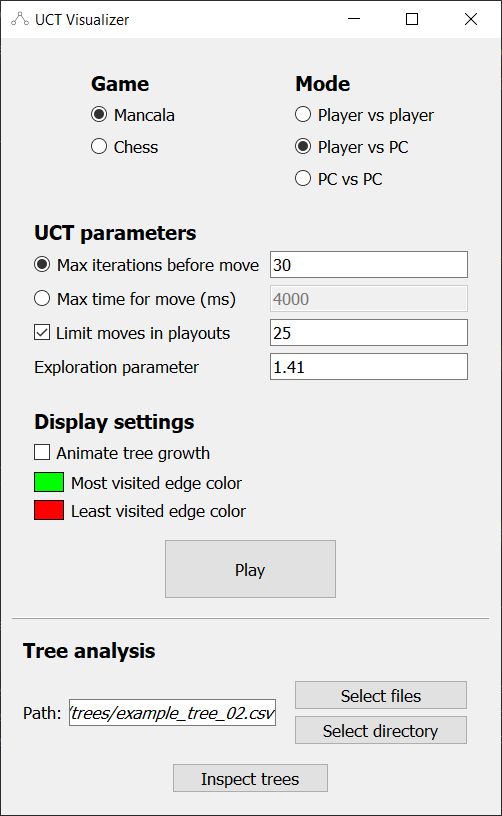
\includegraphics[width=0.55\textwidth]{okno-glowne}
	\caption{Okno menu głównego -- Windows}
	\label{rys:main_menu}
\end{figure}

Z poziomu \textit{Menu głównego} użytkownik może przejść do okien \textit{Rozgrywka} i \textit{Analiza drzewa}. W celu rozegrania gry, należy nacisnąć przycisk \textit{Play}. Powyżej przycisku \textit{Play} znajdują się opcje, które pozwolą użytkownikowi ustawić parametry gry dostosowane do jego preferencji.

\begin{figure}[h!]
	\centering
	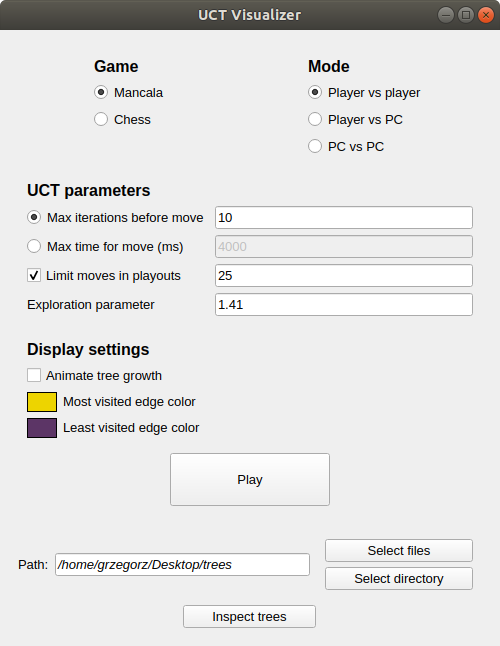
\includegraphics[width=0.6\textwidth]{ubuntu-menu}
	\caption{Okno menu głównego -- Linux}
	\label{rys:main_menu_linux}
\end{figure}

\begin{itemize}
	\item \textbf{Wybór gry} -- do dyspozycji gracza oddane są dwie gry -- szachy i mankala.
	\item \textbf{Wybór trybu rozgrywki} -- użytkownik może wybrać jeden z trzech trybów gry, opisanych poniżej.
	
	\begin{itemize}
		\item Gracz versus PC -- w tym trybie gracz ma okazję zmierzyć się z komputerem, oglądając przy tym generowane drzewa stanów algorytmu UCT.
		\item PC versus PC -- rozgrywka komputera z samym sobą, z możliwością analizowania wynikowych drzew stanów algorytmu. Wybór tego trybu oznacza brak możliwości wykonywania samodzielnych ruchów przez użytkownika, jednakże to od niego będzie zależało, kiedy algorytm wykona kolejny ruch -- będzie miał do dyspozycji przycisk, przy użyciu którego będzie mógł powodować postęp w rozgrywce. 
		\item Gracz versus Gracz -- tryb bez udziału algorytmu UCT, a co za tym idzie, również bez wizualizacji.
	\end{itemize}

	\item \textbf{Wybór liczby iteracji algorytmu} -- liczba powtórzeń wykonania przez algorytm czterofazowej iteracji metody MCTS opisanej w rozdziale \ref{subsec:mcts_group}.
	\item \textbf{Wybór maksymalnego czasu} -- podany w milisekundach; czas, po którym komputer będzie przerywał obliczenia i wykona ruch.
	\item \textbf{Ustawienie limitu ruchów} -- opcjonalne pole, w którym użytkownik może ustalić maksymalną liczbą ruchów w fazie symulacji algorytmu UCT, w celu wcześniejszego kończenia niepożądanie długich rozgrywek.
	\item \textbf{Ustawienie wartości parametru eksploracji} -- pole, w którym użytkownik może ustalić wartość parametru eksploracji algorytmu UCT. Wpływ parametru na działanie algorytmu został opisany w rozdziale \ref{subsec:uct}.
	\item \textbf{Animowanie rozrostu drzewa} -- wybór tej opcji sprawia, że drzewo stanów algorytmu zostaje wyświetlone nie tylko po każdym wykonanym ruchu przez komputer, ale też po każdej iteracji. Co więcej, w panelu po prawej stronie dynamicznie aktualizować się też będzie wartość liczby wszystkich wierzchołków drzewa.
	\item \textbf{Wybór kolorów krawędzi drzewa} -- po kliknięciu na któryś z widocznych kolorów ukaże się paleta systemowa, z której można wybrać inne kolory krawędzi. Najczęściej i najrzadziej odwiedzane węzły drzewa przyjmą wskazane przez użytkownika kolory, inne zaś --- kolory z ich gradientu --- proporcjonalnie do wartości skrajnych licznika odwiedzin.
\end{itemize}

Drugą kluczową opcją dostępną z menu głównego aplikacji jest możliwość przejścia do okna analizy drzewa lub sekwencji drzew. Jest ona dostępna po naciśnięciu przycisku \textit{Inspect trees}. Użytkownik może wczytać pliki z dysku na dwa sposoby: wybierając pliki z folderu bezpośrednio lub wybierając cały katalog, w którym się one znajdują. Do tego celu służą osobno dwa przyciski: \textit{Select files} i \textit{Select directory}, które znajdują się na prawo od pola tekstowego, w którym wyświetlana jest pełna ścieżka do aktualnie wybranego pliku lub katalogu. W przypadku wybrania większej liczby plików, pokazywana jest ich liczność. Można jednocześnie wybierać pliki w formacie CSV i binarnym (.tree), których schemat serializacji został opisany w rozdziale \ref{subsec:serialization}. W przypadku wybrania nieprawidłowego katalogu lub niepoprawnych plików, na ekranie użytkownika pojawi się błąd informujący o problemie, który nastąpił.


\section{Analiza drzewa} \label{subsec:treeanalysis}
W oknie ukazanym na Rysunku \ref{rys:analyze_tree} będziemy mogli oglądać i analizować drzewa wczytane z plików. Ekran podglądu drzewa pozwala w wygodny sposób analizować i porównywać wczytane drzewa oraz udostępnia opcje wymienione poniżej.

\begin{figure}[h!]
	\centering
	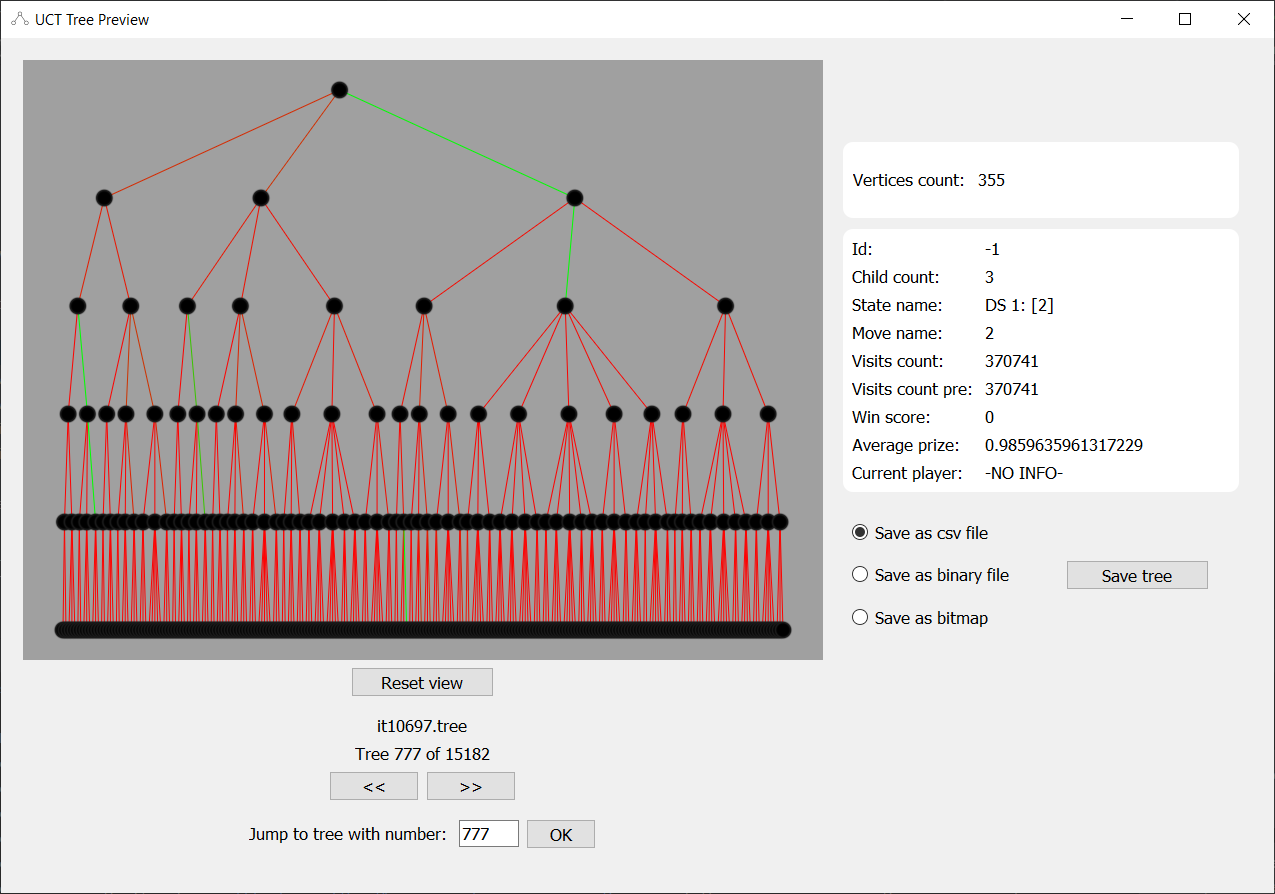
\includegraphics[scale=0.57]{okno-analiza}
	\caption{Okno analizy drzewa}
	\label{rys:analyze_tree}
\end{figure}

\begin{enumerate}
	\item \textbf{Wyświetlenie statystyk węzła} -- po naciśnięciu na węzeł lewym przyciskiem myszy, panel z prawej strony zostaje uzupełniony informacjami, które przechowuje węzeł. Dokładność wykrywania wybranego węzła nie jest zaburzona podczas operowania na przybliżonym lub oddalonym drzewie.
	\item \textbf{Przybliżanie i oddalanie widoku} -- należy naprowadzić kursor na szary obszar drzewa, a następnie przewijać środkowym przyciskiem myszy w górę lub w dół.
	\item \textbf{Przesuwanie drzewa} -- gdy kursor znajduje się w obszarze drzewa, należy nacisnąć prawy przycisk myszy, przytrzymać i poruszać nim na boki w celu przesunięcia widoku całego drzewa.
	\item \textbf{Reset pozycji drzewa} -- pierwotną pozycję i rozmiar drzewa można przywrócić za pomocą przycisku \textit{Reset view} znajdującego się pod widokiem drzewa.
	\item \textbf{Zmiana drzewa w sekwencji} -- jeżeli wczytane zostało więcej niż jedno drzewo, kluczową funkcją jest opcja wygodnego przełączania się między nimi. Można to zrobić na trzy sposoby: używając przycisków ,,<<'' i ,,>>'', które znajdują się w dolnej części okna; klikając lewy i prawy przycisk myszy na klawiaturze (czasami trzeba ustawić uprzednio uaktywnić obszar drzewa, klikając na niego) oraz użycie pola tekstowego, pozwalającego na zmianę aktualnie wyświetlanego drzewa i kliknięcie przycisku \textit{OK}. W przypadku wyświetlania pierwszego lub ostatniego drzewa w sekwencji odpowiednie przyciski strzałek stają się nieaktywne, a w przypadku pola tekstowego ze skokiem następuje walidacja, czy podany numer drzewa mieści się w zakresie.
	\item \textbf{Zapis drzewa} -- możliwość zapisu wyświetlanego drzewa w jednym z trzech dostępnych formatów: CSV, binarnym lub rastrowym (.png). Opcja ta znajduje się z prawej strony okna, pod panelem zawierającym wartości przechowywane przez węzeł. Podczas eksportu do grafiki rastrowej zadbano o to, aby nie występowały artefakty związane z dużym zagęszczeniem krawędzi. Taka grafika zachowuje też aktualne powiększenie i przesunięcie drzewa -- działa na zasadzie zrzutu ekranu.
\end{enumerate}

Co więcej, dla każdego drzewa w sekwencji w panelu dolnym wyświetla się informacja o tym, którym z kolei na liście jest oglądane drzewo oraz jaka jest nazwa pliku, z którego zostało ono wczytane. Dodatkowo, wyświetlana jest liczba wszystkich wczytanych drzew.

\section{Rozgrywka}
\begin{figure}[h!]
	\centering
	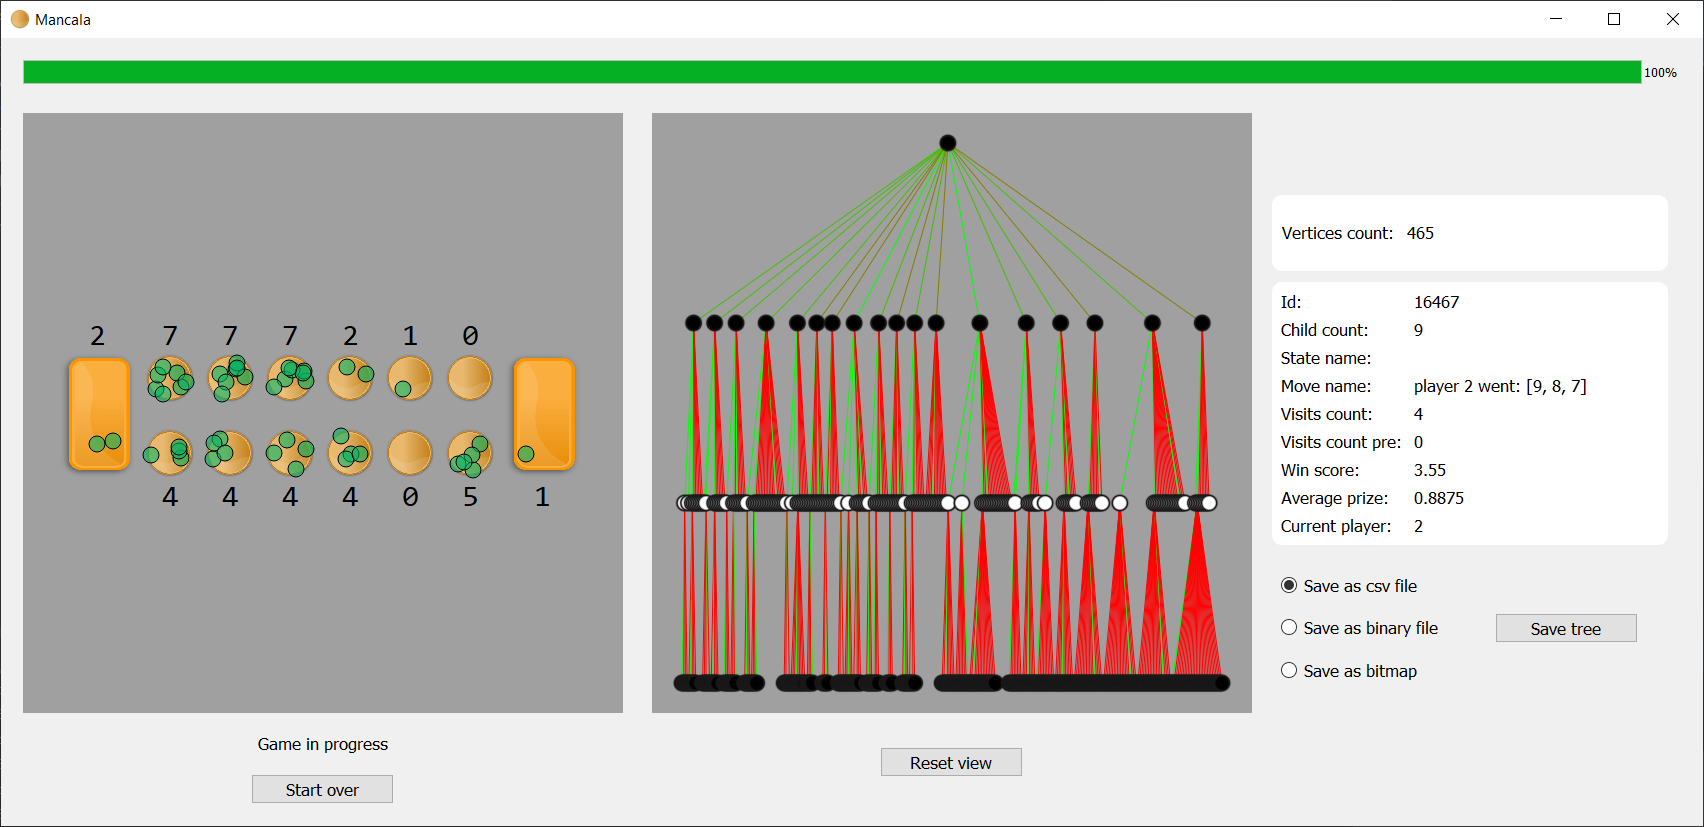
\includegraphics[width=1\textwidth]{okno-mancala}
	\caption{Okno rozgrywki -- mankala, gracz przeciwko PC}
	\label{rys:game_view}
\end{figure}

Na Rysunkach\footnote{Źródło grafik wykorzystanych w mankali: \url{https://www.wpclipart.com/} i w szachach: \url{https://icons8.com/}, na zasadzie \textit{free use}.} \ref{rys:game_view} i \ref{rys:game_view_2} przedstawiony jest interfejs graficzny podczas rozgrywki. Środkową i prawą część okna zajmuje komponent dotyczący analizy drzewa, który został opisany w rozdziale \ref{subsec:treeanalysis}. W związku z tym, wszystkie wyżej opisane funkcjonalności mają zastosowanie również w oknie rozgrywki, poza aspektem dotyczącym sekwencji drzew. Z lewej strony znajduje się panel z wybraną wcześniej grą. Funkcjonalności okna \textit{Rozgrywka} zostały opisane poniżej.
\begin{enumerate}
	\item \textbf{Wykonywanie ruchów} przez gracza, kiedy gra przeciwko PC:
	\begin{itemize}
		\item w przypadku szachów -- wybierając odpowiednią figurę na szachownicy, a następnie jeden z wyświetlonych dostępnych ruchów. Gracz w tym trybie zawsze gra białymi,
		\item w przypadku mankali -- wybierając pewien niepusty dołek z dolnego rzędu planszy.
	\end{itemize}
	\item \textbf{Zrestartowanie gry} przy użyciu przycisku \textit{Start over} w lewej dolnej części okna,
	\item \textbf{Zapisanie drzewa do pliku} przy użyciu przycisku \textit{Save tree}. Format zapisywanego pliku wybierany jest przez zaznaczenie odpowiedniej opcji w liście znajdującej się na lewo od przycisku \textit{Save tree}.
\end{enumerate}

\begin{figure}[h!]
	\centering
	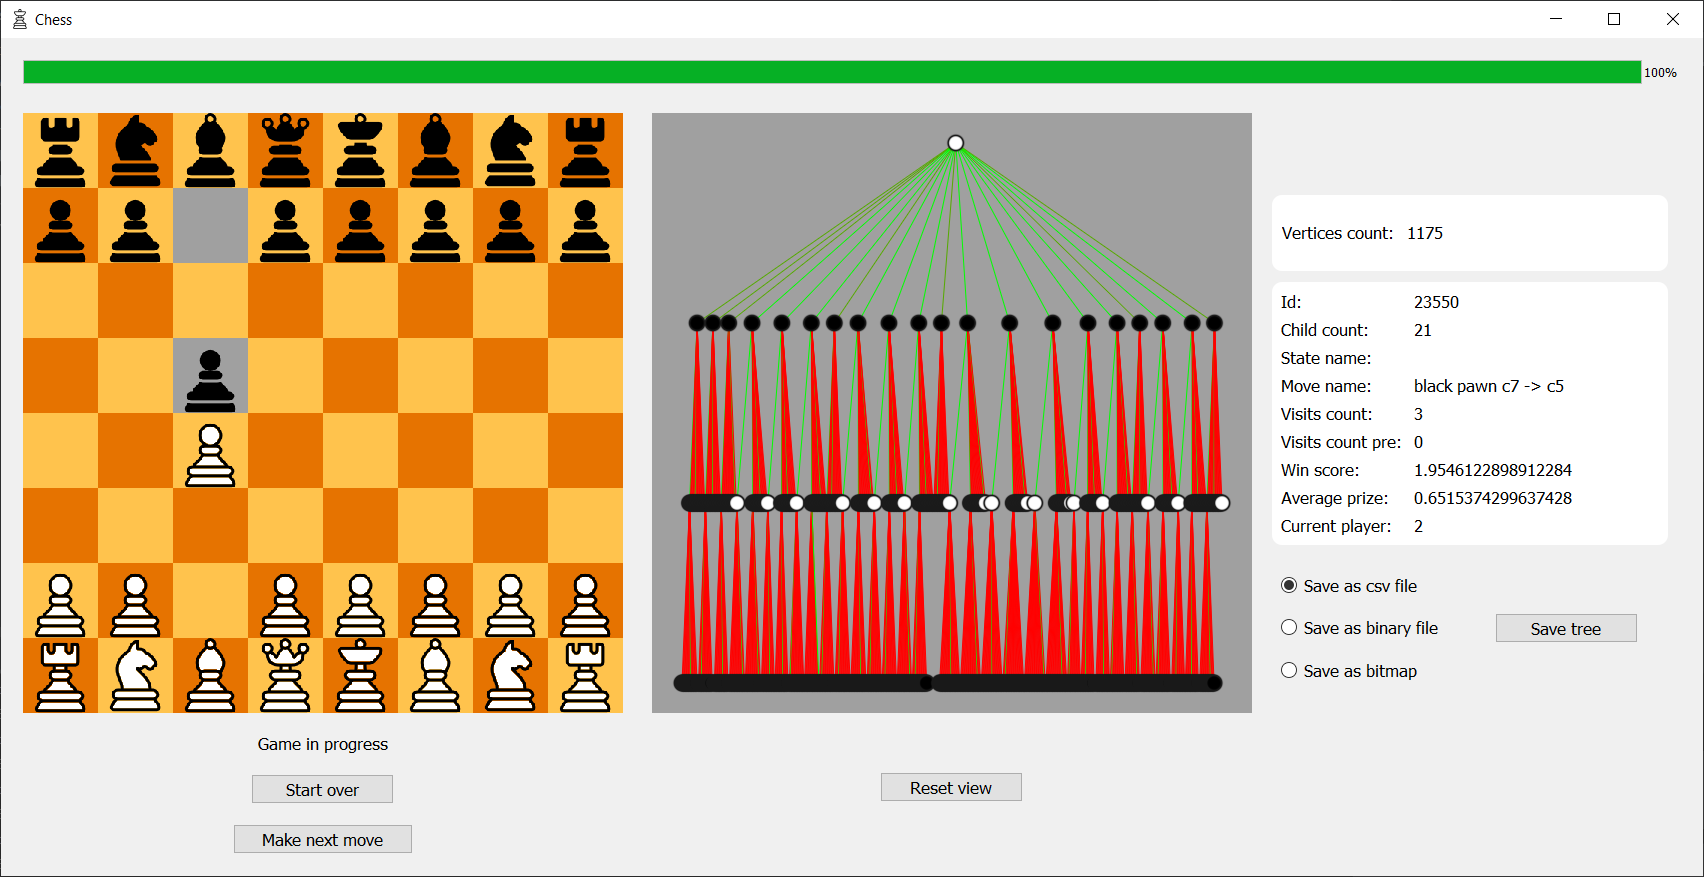
\includegraphics[width=1\textwidth]{okno-szachy}
	\caption{Okno rozgrywki -- szachy, PC przeciwko PC}
	\label{rys:game_view_2}
\end{figure}

Bezpośrednio pod obszarem gry znajduje się etykieta z napisem dotyczącym obecnego stanu rozgrywki. \textit{Game in progress} oznacza, że gra się toczy i wciąż można wykonywać ruchy. W przypadku zakończenia rozgrywki, obszar gry lub przycisk \textit{Make next move} zostaje dezaktywowany i nie można wykonywać kolejnych ruchów aż do ponowienia gry, a etykieta będzie informować o tym, który gracz zwyciężył, wyświetlając napis \textit{Player 1 wins}, \textit{Player 2 wins} lub \textit{Draw}. Przykładowy stan zakończonej gry pokazany jest na Rysunku \ref{rys:game_view_3}.

\begin{figure}[h!]
	\centering
	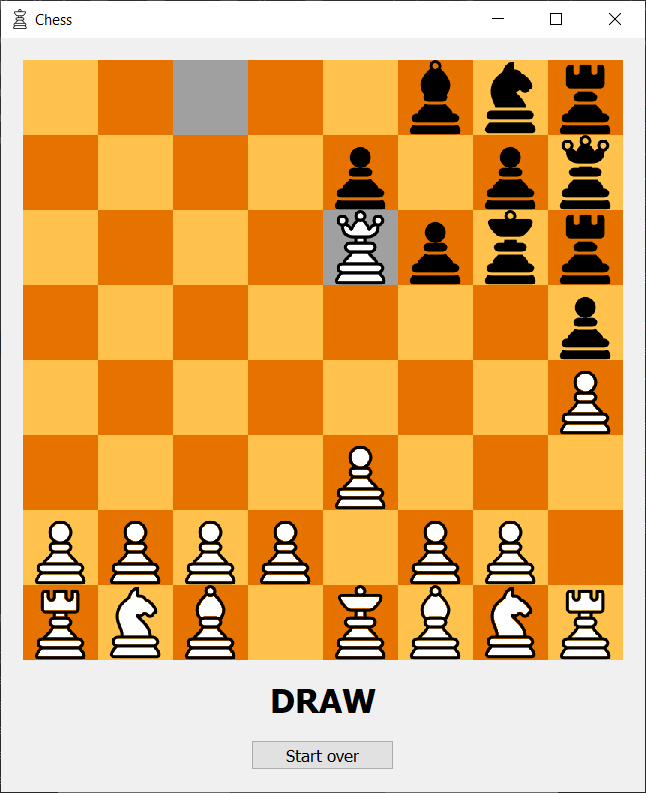
\includegraphics[width=0.6\textwidth]{okno-player-vs-player}
	\caption{Okno rozgrywki -- szachy, dwóch graczy}
	\label{rys:game_view_3}
\end{figure}
